\section{Ejercicio 9}

Para este ejercicio se pedía implementar el scheduler \textit{Multilevel Feedback Queue}, realizar pruebas y mostrar su ejecución.

\subsection{Implementación}

Este scheduler posee n colas \emph{Round Robin} y a cada una de ellas le está asociado un quantum. Estos son recibidos como parámetro.

La estructura que utilizamos es la siguiente:

\begin{itemize}

\item \textbf{colas\_de\_procesos}: vector de colas donde las de mayor prioridad se encuentran en los primeros índices y las de menor en los últimos.

\item \textbf{quantums\_por\_cola}: vector que posee el quantum que tiene cada cola.

\item \textbf{procesos\_corriendo}: una lista de procesos que están corriendo o bloqueados. Un proceso es una estructura en donde tiene su pid, la cola de la que fue tomado y el quantum actual.

\end{itemize}

En el constructor inicializamos los vectores \textbf{colas\_de\_procesos} y \textbf{quantums\_por\_cola}. Mientras haya quantums en el vector que se recibe como parámetro se van agregando colas a \textbf{colas\_de\_procesos} y el quantum en \textbf{quantums\_por\_cola}.

En la función \textbf{load}, el nuevo proceso es cargado en la cola de mayor prioridad (índice 0) de \textbf{colas\_de\_procesos}.

En la función \textbf{unblock}, se busca el proceso en la lista \textbf{procesos\_corriendo} para ver de que cola fue tomado y se lo inserta en la siguiente (salvo que sea la última, si lo es se queda en ella). Luego se lo elimina de la lista.

La función \textbf{tick} tiene un comportamiento mas complicado que pasamos a detallar en el siguiente pseudocódigo:

~

\begin{algorithmic}
\Function{int tick}{int cpu, const enum Motivo m}

	\If {\emph{Si la tarea actual es la IDLE\_TASK y hay procesos en alguna cola}}
		\State Desencolo el proceso de cola de mayor prioridad.
		\State Agrego el proceso en la lista.
		\State Lo devuelvo.
		
	
	\ElsIf{\emph{Si el motivo fue un TICK}}
		\State Actualizo el quantum de la tarea.

		\If{\emph{Si terminó su quantum y hay otros procesos encolados.}}
			\State Quito el proceso actual de la lista \textbf{procesos\_corriendo}. Y lo encolo en la siguiente cola.
			\State Tomo el nuevo proceso de la cola de mayor prioridad, lo agrego a la lista \textbf{procesos\_corriendo} y lo devuelvo.

		\ElsIf{\emph{Si terminó su quantum y no hay otros procesos encolados.}}
			\State Actualizo el quantum y lo devuelvo.

		\EndIf

	\ElsIf{\emph{Si el motivo fue un EXIT y hay procesos encolados}}
		\State Elimino el proceso que termino de la lista \textbf{procesos\_corriendo}.
		\State Desencolo el proceso de cola de mayor prioridad.
		\State Agrego el proceso en la lista.
		\State Lo devuelvo.

	\ElsIf{\emph{Si el motivo fue un BLOCK y hay procesos encolados}}
		\State Desencolo el proceso de cola de mayor prioridad.
		\State Agrego el proceso en la lista.
		\State Lo devuelvo.
	
	\Else
		\State Devuelvo IDLE\_TASK.

	\EndIf
\EndFunction	
\end{algorithmic}

\subsection{Pruebas}

Para estas pruebas generamos un lote (\textit{ej9lote}) que posee cinco tareas de los tipos TaskConsola, TaskIO, TaskBatch y TaskCPU. Estas son lanzadas desde el comienzo con una diferencia de dos clocks cada una. La cantidad de cores es de uno, el costo del cambio de contexto es de dos y el costo de cambiar un proceso de núcleo es de uno.

En este caso, tenemos tres colas de quantums decrecientes (6, 4 y 2), crecientes (2, 4 y 6) y constantes (3, 3 y 3). Veamos cómo se comportan:

\begin{figure}[!h]
	\begin{center}
		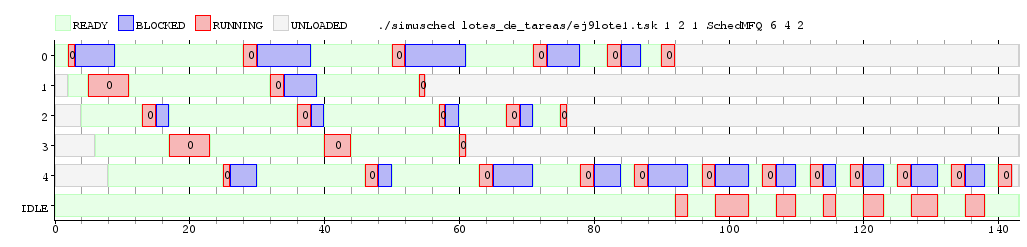
\includegraphics[width=500px]{imagenes/ej9_1.png}
		\caption{Ejecución del lote \emph{ej9lote} con tres colas de quantum decreciente.}
		\label{fig:grafico_ej9_1}
	\end{center}
\end{figure}

\begin{figure}[!h]
	\begin{center}
		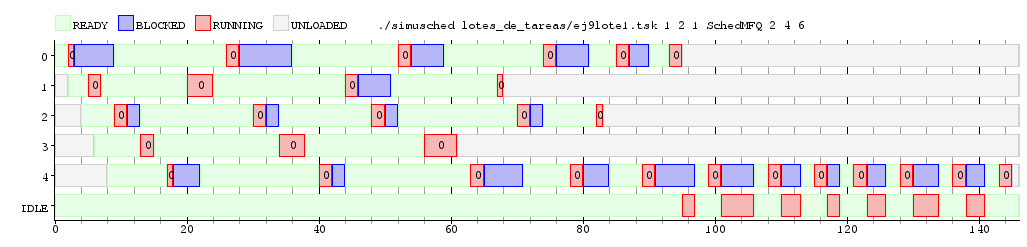
\includegraphics[width=500px]{imagenes/ej9_2.png}
		\caption{Ejecución del lote \emph{ej9lote} con tres colas de quantum creciente.}
		\label{fig:grafico_ej9_2}
	\end{center}
\end{figure}

\begin{figure}[!h]
	\begin{center}
		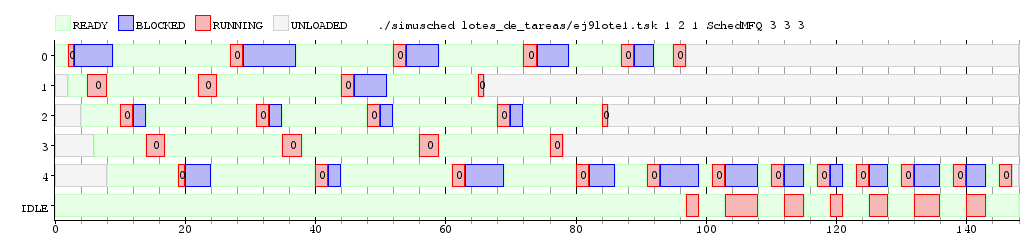
\includegraphics[width=500px]{imagenes/ej9_3.png}
		\caption{Ejecución del lote \emph{ej9lote} con tres colas con quantum 3.}
		\label{fig:grafico_ej9_3}
	\end{center}
\end{figure}

%LATENCIA PROMEDIO
\begin{center}
	\begin{tabular}{|c|c|c|}
		\hline
		\multicolumn{3}{|c|}{\large{\textbf{Latencia Promedio}}} \\
		\hline
		\textbf{Quantum Decreciente} & \textbf{Quantum Creciente} & \textbf{Quantum Estable} \\
		\hline
		8,4 & 5,2 & 6 \\
		\hline
	\end{tabular}
\end{center}

%WAITING TIME PROMEDIO
\begin{center}
	\begin{tabular}{|c|c|c|}
		\hline
		\multicolumn{3}{|c|}{\large{\textbf{Waiting Time Promedio}}} \\
		\hline
		\textbf{Quantum Decreciente} & \textbf{Quantum Creciente} & \textbf{Quantum Estable} \\
		\hline
		50,2 & 57,4 & 58 \\
		\hline
	\end{tabular}
\end{center}

%TIEMPO TOTAL DE EJECUCION PROMEDIO
\begin{center}
	\begin{tabular}{|c|c|c|}
		\hline
		\multicolumn{3}{|c|}{\large{\textbf{Tiempo Total De Ejecución Promedio}}} \\
		\hline
		\textbf{Quantum Decreciente} & \textbf{Quantum Creciente} & \textbf{Quantum Estable} \\
		\hline
		81,6 & 86,4 & 90,6 \\
		\hline
	\end{tabular}
\end{center}

Cómo podemos observar en esta prueba, tener un quantum decreciente hace que la latencia sea la mayor, pero genera un waiting time y tiempo total de ejecución menores que las otras dos ejecuciones con quantum creciente y quantum estable. Tener un quantum creciente genera que su latencia promedio sea la menor pero con waiting time promedio y tiempo de ejecución promedio mucho mayores. Tener un quantum estable genera que este scheduler sea cómo un \textbf{Round Robin} común ya que no se diferencian las prioridades de las colas que pueda poseer.

Este scheduler resulta interesante para analizar y comparar contra los otros schedulers vistos en este trabajo ya que podría mejorar la performance de estos. 
